% Chapter Template

\chapter{Methodology} % Main chapter title

\label{Chapter3} % Change X to a consecutive number; for referencing this chapter elsewhere, use \ref{ChapterX}

\lhead{Chapter 3. \emph{Methodology}} % Change X to a consecutive number; this is for the header on each page - perhaps a shortened title

%----------------------------------------------------------------------------------------
%	INTRO
%----------------------------------------------------------------------------------------


Three essential blocks form a sensor network. Namely sensors, processors and communication devices\citep{chong2003sensor}. In the next sections all of them will be explained and in the next chapter I will show how are these related. There is even a case where a device (Digi XBee\textregistered) fulfills two of these roles.


%----------------------------------------------------------------------------------------
%	SECTION 1
%----------------------------------------------------------------------------------------

\section{Sensors}

We now live in a world where we hear a lot the word ``sensor'', but what is exactly a sensor? \emph{A sensor is a converter that measures a physical quantity and converts it into a signal which can be read by an observer or by an instrument.}\citep{WikiSensor}

This might (and is) quite simple, but complexity resides on calibration and coming up with actual useful applications. Since every sensor from the same family is equal in terms of design but different in reality (due to small random variations during the fabrication process) output has to be adjusted to agree with a given standard. When it comes to applications, RFID tags can be used to determine wether a book is on the right spot in a library or not, or with a very intense light beam we can detect how the blood flows through a vein thus succesfully sensing heart rate. These are just two imaginative uses for nowaday sensors.

In the first (and only at the time) iteration of this pilot only environmental factors have been measured since those have been tested over and over for the last years and they serve as a proof of concept for this network.

%-----------------------------------
%	SUBSECTION 1 - DHT22
%-----------------------------------
\subsection{Aosong DHT22\citep{dht22sensor}}

The DHT22 is a low cost humidity and temperature sensor designed by Aosong Electronics, a Chinese corporation. This is a digital sensor, which means that the output is represented in the form of bits, thus requiring some amount of computational power to ``interpret'' the results. The output format is precisely described in the datasheet of this product, and luckily there already are some library implementations to work with the DHT22. Then, this device will only work with platforms that allow digital input, such Arduino.

\begin{figure}[htbp]
    \centering
        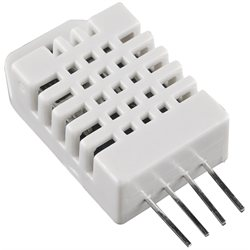
\includegraphics[scale=0.8]{./Figures/dht22.jpg}
        \rule{35em}{0.5pt}
    \caption[DHT22 sensor]{DHT22 humidity and temperature sensor.}
    \label{fig:DHT22}
\end{figure}


%------------------------------------
%	SUBSECTION 2 - MINI SOUND SENSOR
%------------------------------------

\subsection{Emartee Mini Sound Sensor\citep{emarteeminisound}}

Manufactured by Emartee, can also be found by the name of ``Emartee part number 4021'', and can be used to measure noise levels among other uses. Esentially, it consists on a microfone with a built-in amplifier onto a breakout board, which can be useful to work directly with perfboards or breadboards (both construction bases for rapid prototyping of electronic circuits).

The output signal is analog and is increased by a factor that allows an Arduino or any device with analog I/O pins to detect it easily\citep{gertz2012environmental}. Its operating voltage is 5V.


%------------------------------------
%	SUBSECTION 3 - SHARP DUST
%------------------------------------

\subsection{Sharp GP2Y1010AU0F\citep{sharp}}

This is an inexpensive optical dust sensor, used to measure air quality. It is made out of an infrarred emitting diode which with a well positioned phototransistor can measure the reflected IR rays thus detecting dust levels in the air. This device, which can be powered with up to 7V gives an output voltage (analog) proportional to dust density in the air. Some of its applications are air monitoring and air conditioning.

\begin{figure}[htbp]
    \centering
        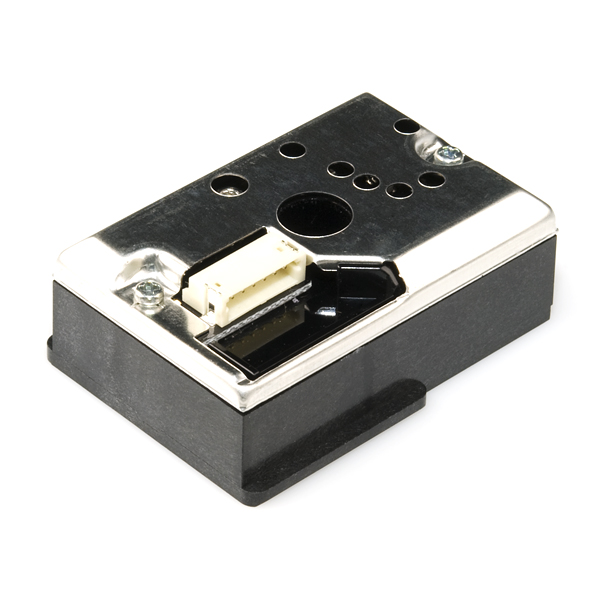
\includegraphics{./Figures/sharp.jpg}
        \rule{35em}{0.5pt}
    \caption[Sharp GP2Y1010AU0F]{Sharp GP2Y1010AU0F optical dust sensor.}
    \label{fig:SharpGP2Y1010AU0F}
\end{figure}

Surprisingly, this detector, which is worth at the time of writing about \$12, gives very precise results, similar to those offered by an expensive laser particle counter.\citep{airquality}


%----------------------------------------------------------------------------------------
%	SECTION 2 - XBEE MODULE
%----------------------------------------------------------------------------------------

\section{Digi XBee\textregistered{} Wireless RF Module\citep{xbeedatasheet}}

These radio modules are based on the IEEE 802.14.4 standard and provide an unexpensive, low power, low rate communication. They mainly use ISM bands. Despite their size provide us with many interesting features, such as 128-bit encryption, over-the-air configuration and ADC/digital input/output pins.

\begin{figure}[htbp]
    \centering
    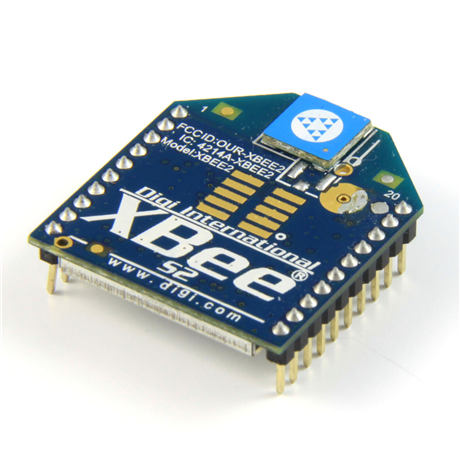
\includegraphics[scale=0.4]{./Figures/xbee.png}
        \rule{35em}{0.5pt}
        \caption[Digi XBee RF Module]{Digi XBee\textregistered{} Wireless RF Module}
    \label{fig:XBee RF Module}
\end{figure}

There are two versions of these modules, named ``Series 1'' and ``Series 2''. The older one (Series 1) implements the previously mentioned IEEE 802.15.4 standard which allows point to point (or star) topologies. On the other hand however, the latter implements a standard specification called \emph{ZigBee}. This protocol, although more complex has mesh networking capabilities which can be a key feature in some sensor networks.

This is why for the sake of this project ``Series 2'' has been chosen. It is worth saying that each of the two versions can transmit with different power levels thus varying the effective communication range\citep{faludi2010building}. More detailed information can be found in the table below.

% -T-A-B-L-E---- 
\begin{table}[ht] 
\centering
\begin{tabular}{l l l l}
    Version     & Power                 & Indoor range     & LoS range\footnotemark[1]\\
\hline
Series 1        & 1mW                   & 30m              & 100m\\
Series 1 PRO    & 63mW\footnotemark[2]  & 90m              & 1600m\\
Series 2        & 2mW                   & 40m              & 120m\\
Series 2 PRO    & 63mW\footnotemark[2]  & 90m              & 1500m\\
\end{tabular}
\caption{Comparison of different versions of XBee\textregistered.}
\end{table}

\footnotetext[1]{LoS range refers to line of sight range, where a straight line can be drawn from the transmitter to the receiver. In this situation, there are no obstacles between them and better bitrates and/or ranges can be achieved.}
\footnotetext[2]{This output power can be obtained using high gain antennas.}

Also, if extra range is needed (up to 40km in line of sight) there are also XBee\textregistered{} devices that transmit in lower ISM bands (900 and 868 MHz). However, when transmitting in these frequencies neither ZigBee nor IEEE 802.15.4 can be used. DigiMesh\texttrademark{} networking protocol is the only option and it is property of Digi International Inc.


%----------------------------------------------------------------------------------------
%	SECTION 3 - ARDUINO
%----------------------------------------------------------------------------------------

\section{Arduino}

Arduino is the leading protopying platform nowadays. It is completely open source including the schematics of the hardware itself, which is a single-board microcontroller. Anyone can program the board through a programming language very similar to C/C++ and based on \href{http://wiring.org.co}{Wiring}. To upload a sketch (a program) to the microcontroller they also have developed an Arduino IDE based on \href{htpp://processing.org}{Processing}.

The amount of projects related to this platform is incredibly big, and it has gained huge popularity amongst designers, hackers, programmers and hobbyists these past years. It offers several advantages over similar devices, because it is really cheap, cross-platform and has every benefit inherent to the open source initiative. Also, like other open projects Arduino comes in many ``flavours'' depending on the characteristics of the project.

As it can be seen on the next picture, the board has many input/output pins that are compatible with analog and digital values. It's not just that but also it can establish a serial communication with a computer so interaction between programs and the platform can take place.


\begin{figure}[htbp]
    \centering
    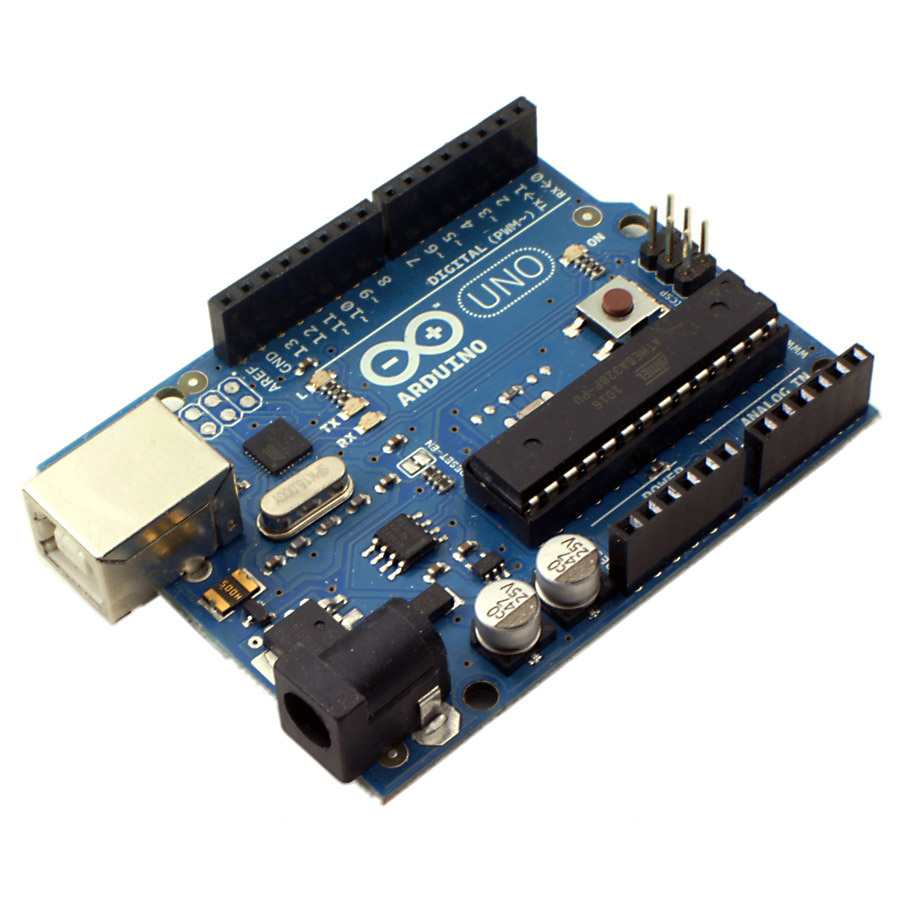
\includegraphics[scale=0.2]{./Figures/auno.jpg}
        \rule{35em}{0.5pt}
        \caption[Arduino UNO]{Arduino UNO prototyping platform.}
    \label{fig:ArduinoUNO}
\end{figure}

Arduino UNO is the one ``flavour'' that has been chosen to perform this project, since it is cheap and also the most common. That means all shields\footnote{A shield is another board plugged on top of the Arduino to extend its functionalities.}  work by default on it and the community is the biggest. In particular, this model has the following features\citep{arduinounor3}:
\\

\begin{table}[ht] 
\centering
\begin{tabular}{l|l}
    Feature     & Value\\
\hline
Microcontroller	& ATmega328\\
Operating Voltage &	5V\\
Input Voltage (recommended) & 7-12V\\
Input Voltage (limits) & 6-20V\\
Digital I/O Pins & 14 (of which 6 provide PWM output)\\
Analog Input Pins & 6\\
DC Current per I/O Pin & 40 mA\\
DC Current for 3.3V Pin & 50 mA\\
Flash Memory & 32 KB (ATmega328) of which 0.5 KB used by bootloader\\
SRAM & KB (ATmega328)\\
EEPROM &	1 KB (ATmega328)\\
Clock Speed &	16 MHz\\
\end{tabular}
\caption{Characteristics of the Arduino UNO.}
\end{table}
